\documentclass[12pt, a4paper]{article}
\input{../format.tex}  

\begin{document}
	\onehalfspacing
	Date: \today{} \hfill{} Name: Maitreya Ranade
	\begin{center}
		\topskip0pt
		\vspace*{\fill}
		{\LARGE C++ Language} \\
		% This report is written for personal understanding and not for publication or distribution.
		\vspace*{\fill}
	\end{center}
	
	\pagebreak
	\singlespacing
	\tableofcontents
	\pagebreak
	
    \chapter{C Programming}

    \section{Introduction}
    \input{introduction.tex}
    \clearpage
    
    \section{Variables}
    \input{variables.tex}
    \clearpage

    \section{Constants}
    \begin{itemize}
        \item Constant is something that never changes. In other words, once defined cannot be modified later in the code.
        \item \#define is a preprocessor directive.
        \begin{itemize}
            \item Syntax: \#define name value (name is also called macro)
            \item Avoid semicolon at the end in the syntax.
            \item Choosing capital letters for name is good practice.
            \item Preprocessor replaces Name with value.
            \item We can use macros like functions.
            \item First expansion then evaluation.
            \item There are current predefined / standard Macros ex. \_\_TIME\_\_ \& \_\_DATE\_\_.
        \end{itemize}
        \item Const keyword
        \begin{itemize}
            \item A variable defined with the const modifier are considered variables, and not macro definitions. 
            \item syntax: const data\_type variable\_name
        \end{itemize}
        \item Const-s are handled by the compiler, where as \#define-s are handled by the pre-processor.
        \item The big advantage of const-s over \#define is type checking. \#define-s can't be type checked.
        \item Since const-s are considered variables, we can use pointers on them. This means we can typecast, move addresses, and everything else you'd be able to do with a regular variable besides change the data itself, since the data assigned to that variable is constant.
    \end{itemize}

    \clearpage

    \section{Memory Layout of C program}
    A typical memory representation of a C program consists of the following sections.
    \begin{enumerate}
        \item Text/Code segment  
        \item Initialized data segment 
        \item Uninitialized data segment  (bss)
        \item Heap 
        \item Stack
    \end{enumerate}

    \begin{figure}[H]
        \begin{center}
            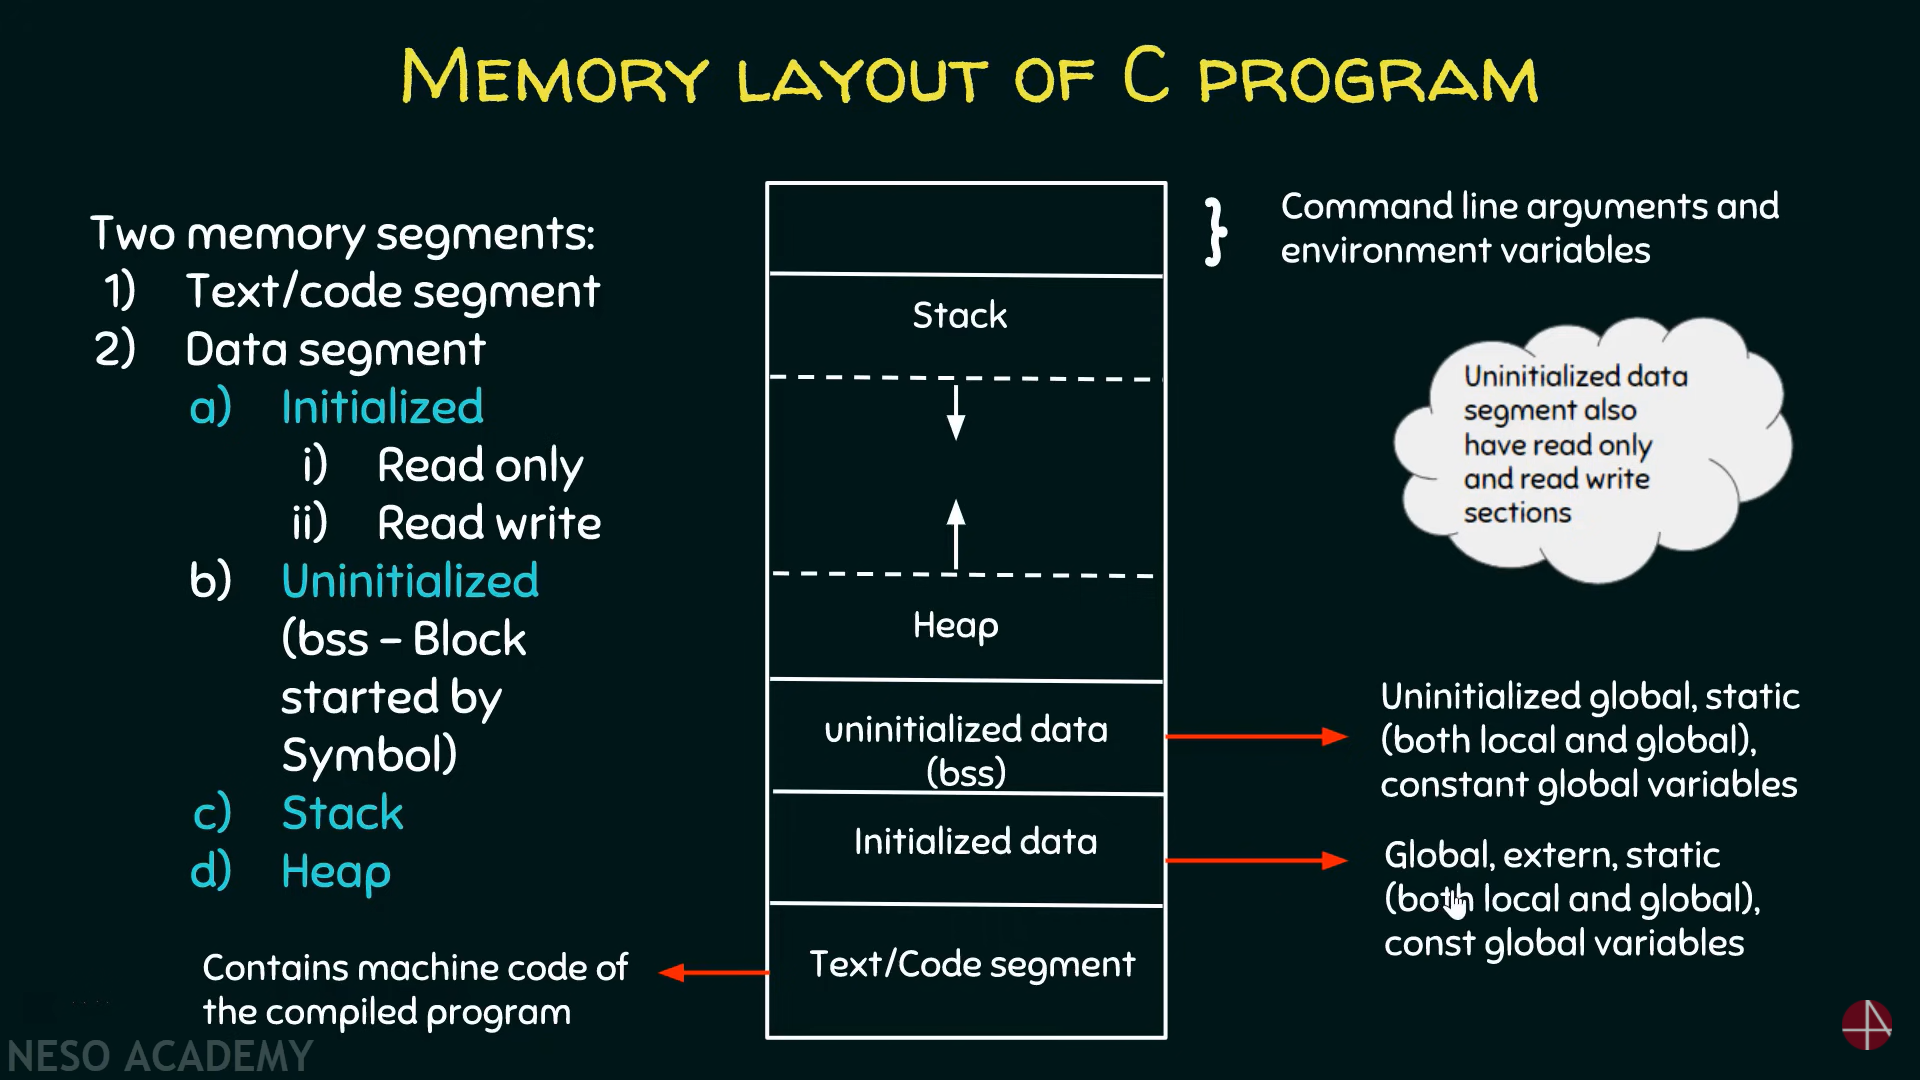
\includegraphics[width=0.6\textwidth]{images/memoryLayoutC.png}
            \caption{Memory Layout of C program}
            \label{memoryLayoutC}
        \end{center}
    \end{figure}

    C program gets stored into not one but multiple sections of the memory. A typical memory layout of a running process is as follows:
    \subsection{Text/Code segment}
    \begin{itemize}
        \item A text segment, also known as a code segment or simply as text, contains machine code of the compiled program or executable instructions.
        \item The text segment is often read-only, to prevent a program from accidentally modifying its instructions.        
        \item As a memory region, a text segment may be placed below the heap or stack in order to prevent heaps and stack overflows from overwriting it.         
        \item Usually, the text segment is sharable so that only a single copy needs to be in memory for frequently executed programs, such as text editors, the C compiler, the shells, and so on. 
    \end{itemize}   
    
    \subsection{Initialized Data Segment}
    \begin{itemize}
        \item Initialized data segment, usually called simply the Data Segment. 
        \item A data segment is a portion of the virtual address space of a program, which contains the global, extern, static (local and global), and const global variables that are initialized by the programmer.
        \item Note that, the data segment is not read-only, since the values of the variables can be altered at run time.    
        \item This segment can be further classified into the read-only (for const-s) area and the read-write sections.
    \end{itemize}
    
    \subsection{Uninitialized Data Segment}
    \begin{itemize}
        \item Uninitialized data segment often called the "bss" segment, named after an ancient assembler operator that stood for "block started by symbol".
        \item Uninitialized data segment contains all uninitialized global, static(local and global), and constant global variables.
        \item Data in this segment is initialized by the kernel to arithmetic 0 before the program starts executing.    
        \item This segment is also further classified into read-only (for const-s) area and read-write sections.             
    \end{itemize}
    
    \subsection{Stack}
    The stack area traditionally adjoined the heap area and grew in the opposite direction; when the stack pointer met the heap pointer, free memory was exhausted. (With modern large address spaces and virtual memory techniques they may be placed almost anywhere, but they still typically grow in opposite directions.)

    The stack area contains the program stack, a LIFO structure, typically located in the higher parts of memory. On the standard PC x86 computer architecture, it grows toward address zero; on some other architectures, it grows in the opposite direction. A "stack pointer" register tracks the top of the stack; it is adjusted each time a value is "pushed" onto the stack. The set of values pushed for one function call is termed a "stack frame"; A stack frame consists at minimum of a return address.

    Stack, where automatic variables are stored, along with information that is saved each time a function is called. Each time a function is called, the address of where to return to and certain information about the caller's environment, such as some of the machine registers, are saved on the stack. The newly called function then allocates room on the stack for its automatic and temporary variables. This is how recursive functions in C can work. Each time a recursive function calls itself, a new stack frame is used, so one set of variables doesn't interfere with the variables from another instance of the function.
    
    \subsection{Heap}
    Heap is the segment where dynamic memory allocation usually takes place.
    
    The heap area begins at the end of the BSS segment and grows to larger addresses from there. The Heap area is managed by malloc, realloc, and free, which may use the brk and sbrk system calls to adjust its size (note that the use of brk/sbrk and a single "heap area" is not required to fulfill the contract of malloc/realloc/free; they may also be implemented using mmap to reserve potentially non-contiguous regions of virtual memory into the process' virtual address space). The Heap area is shared by all shared libraries and dynamically loaded modules in a process.

    \clearpage


    \section{Operators}
    \input{operators.tex}
    \clearpage
    
    \section{Conditionals}
    \input{conditionals.tex}
    \clearpage
    
    \section{Loops}
    \input{loops.tex}
    \clearpage

    \section{Functions \& Pointers}
    \input{pointers.tex}
    \clearpage    
    
    \section{C/C++ Preprocessors}

    As the name suggests Preprocessors are programs that process our source code before compilation. There are a number of steps involved between writing a program and executing a program in C / C++. 


    \begin{figure}[H]
        \begin{center}
            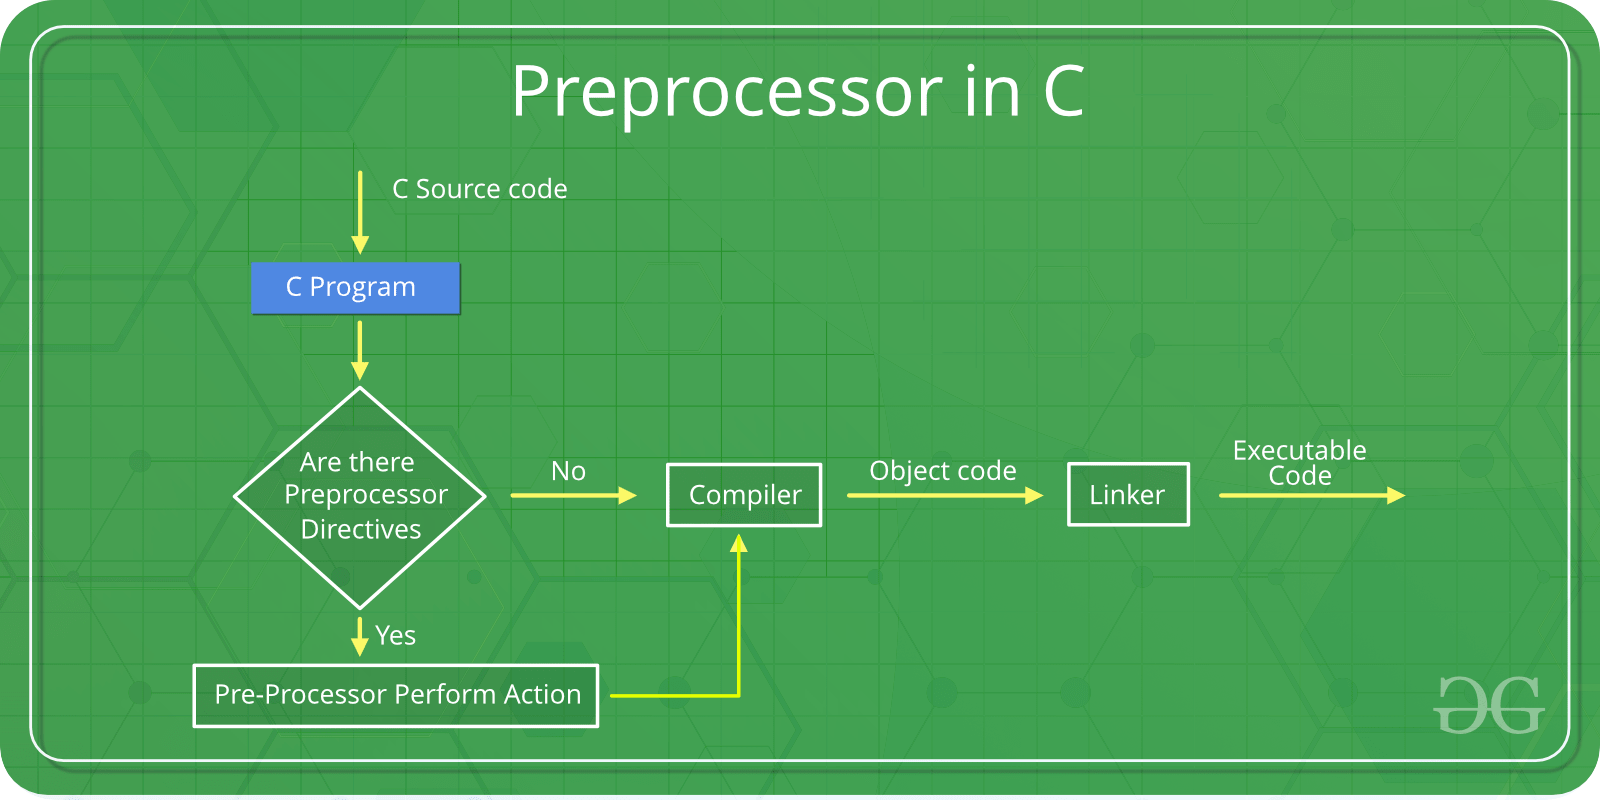
\includegraphics[width=0.6\textwidth]{images/Cpreprocessor.png}
            \caption{Preprocessor in C}
            \label{Cpreprocessor}
        \end{center}
    \end{figure}

    The source code file is processed by preprocessors and an expanded source code file is generated named program. This expanded file is compiled by the compiler and an object code file is generated named program .obj. Finally, the linker links this object code file to the object code of the library functions to generate the executable file program.exe.

    \par Preprocessor programs provide preprocessors directives which tell the compiler to preprocess the source code before compiling. All of these preprocessor directives begin with a '\#' (hash) symbol. The '\#' symbol indicates that, whatever statement starts with \#, is going to the preprocessor program, and preprocessor program will execute this statement. Examples of some preprocessor directives are: \#include, \#define, \#ifndef etc. Remember that \# symbol only provides a path that it will go to the preprocessor, and command such as include is processed by preprocessor program. For example, include will include extra code to your program. We can place these preprocessor directives anywhere in our program. 

    There are 4 main types of preprocessor directives: 
    \begin{enumerate}
        \item Macros
        \item File Inclusion
        \item Conditional Compilation
        \item Other directives
    \end{enumerate} 
    
    Macros: Macros are a piece of code in a program which is given some name. Whenever this name is encountered by the compiler the compiler replaces the name with the actual piece of code. The '\#define' directive is used to define a macro. 

    \begin{highlight}
        Note: There is no semi-colon(';') at the end of macro definition. Macro definitions do not need a semi-colon to end.
    \end{highlight}


    File Inclusion: This type of preprocessor directive tells the compiler to include a file in the source code program. There are two types of files which can be included by the user in the program: 
        Header File or Standard files: These files contains definition of pre-defined functions like printf(), scanf() etc. These files must be included for working with these functions. Different function are declared in different header files. For example standard I/O functions are in 'iostream' file whereas functions which perform string operations are in 'string' file.
        
        user defined files: When a program becomes very large, it is good practice to divide it into smaller files and include whenever needed. These types of files are user defined files. These files can be included as:


    Conditional Compilation: Conditional Compilation directives are type of directives which helps to compile a specific portion of the program or to skip compilation of some specific part of the program based on some conditions. This can be done with the help of two preprocessing commands 'ifdef' and 'endif'. 

    If the macro with name as 'macroname' is defined then the block of statements will execute normally but if it is not defined, the compiler will simply skip this block of statements. 

    Other directives: Apart from the above directives there are two more directives which are not commonly used. These are: 
    \#undef Directive: The \#undef directive is used to undefine an existing macro. This directive works as:

    Using this statement will undefine the existing macro LIMIT. After this statement every “\#ifdef LIMIT” statement will evaluate to false. 

    \#pragma Directive: This directive is a special purpose directive and is used to turn on or off some features. This type of directives are compiler-specific, i.e., they vary from compiler to compiler. Some of the \#pragma directives are discussed below: 
    \#pragma startup and \#pragma exit: These directives helps us to specify the functions that are needed to run before program startup( before the control passes to main()) and just before program exit (just before the control returns from main()). 
    Note: Below program will not work with GCC compilers. 
    Look at the below program:


    \#pragma warn Directive: This directive is used to hide the warning message which are displayed during compilation. 
    We can hide the warnings as shown below: 
    \#pragma warn -rvl: This directive hides those warning which are raised when a function which is supposed to return a value does not returns a value.
    \#pragma warn -par: This directive hides those warning which are raised when a function does not uses the parameters passed to it.
    \#pragma warn -rch: This directive hides those warning which are raised when a code is unreachable. For example: any code written after the return statement in a function is unreachable.


    \paragraph{Pragma Directive in C/C++}
    This directive is a special purpose directive and is used to turn on or off some features. This type of directives are compiler-specific i.e., they vary from compiler to compiler. Some of the pragma directives are discussed below:
    
    \#pragma startup and \#pragma exit: These directives helps us to specify the functions that are needed to run before program startup( before the control passes to main()) and just before program exit (just before the control returns from main()).
    Note: Below program will not work with GCC compilers.
    Look at the below program:
    
    \iffalse
        https://www.tutorialspoint.com/c-cplusplus-preprocessor-directives
        https://www.tutorialspoint.com/cplusplus/cpp_preprocessor.htm
        https://www.geeksforgeeks.org/cc-preprocessors/
        https://www.tutorialspoint.com/cprogramming/c_preprocessors.htm
    \fi


    \iffalse
    \section{Recursion}
    \section{Arrays}
    \section{Structure and union}
    \section{File handling}


    \chapter{Data Structures}    
    \section{Introduction}
    \section{Stacks}
    \section{Queues}
    \section{Linked Lists}
    \section{Trees}
    \section{Binary Search Trees}
    \section{Binary Heaps}
    \section{Graphs}

	\fi

    % \section{Programs in C}
    % \input{programs.tex}
    % \clearpage

    \section{References}

	\begin{itemize} 
        \item \href{https://youtube.com/playlist?list=PLBlnK6fEyqRhX6r2uhhlubuF5QextdCSM}{Neso Academy (Youtube Channel) (C Programming \& Data Structures playlist)}
        \item Let us C by Yashwant Kanetkar    
        \item \href{https://www.tutorialspoint.com/cprogramming/index.htm}{Tutorials Point}
        \item \href{https://www.geeksforgeeks.org/c-programming-language/}{Geeks for geeks}
        \item \href{https://publications.gbdirect.co.uk/c_book/}{The C book}
	\end{itemize}
	
\end{document}




